\begin{apendicesenv}

\partapendices

\chapter{Código do Transmissor}


O código do transmissor de dados é apresentado citação [\ref{Transmissor_MSP}]. Este código foi desenvolvido para o microcontrolador MSP430. Foi utilizado um clock de 1 MHz. O qual foi dividido para fornecer 100 Hz para sincronizar o transmissor e receptor.
A mesagem a ser transmitida está contida dentro do código.



\lstinputlisting[language=C, caption={Código do transmissor MSP430.}, label={Transmissor_MSP}]{codigos/main.c}



\chapter{Código Do Receptor}

Este código foi projetado para rodar no microcontrolador Atmega 328, e está configurado para receber pacote de mensagens de 12bits. O controlador colhe um novo bit a cada 5 ms como aprsentado no código [\ref{Receptor_arduino}]. 



\lstinputlisting[language=C, caption={Código do Receptor Arduino.}, label={Receptor_arduino}]{codigos/receptor/receptor.ino}

\chapter{Cronograma de execução Tcc2}

Os cronogramas apresentados abaixo nas figuras [\ref{Fig: Network_diagram} e \ref{Fig: Grantt_diagram}] explicita o trabalho a ser desenvolvido no TCC 2. A segunda versão deste trabalho terá como foco um melhor desenvolvimento de \textit{hardware} que possibilite maiores taxas de transmissão assim como maior área de cobertura da rede. Por este motivo busca-se aprimorar os \textit{hardwares} de detecção e transmissão. E como resultado o \textit{software} de suporte deverá ser adaptado as novas configurações do sistema.

\begin{figure}
	\centering
		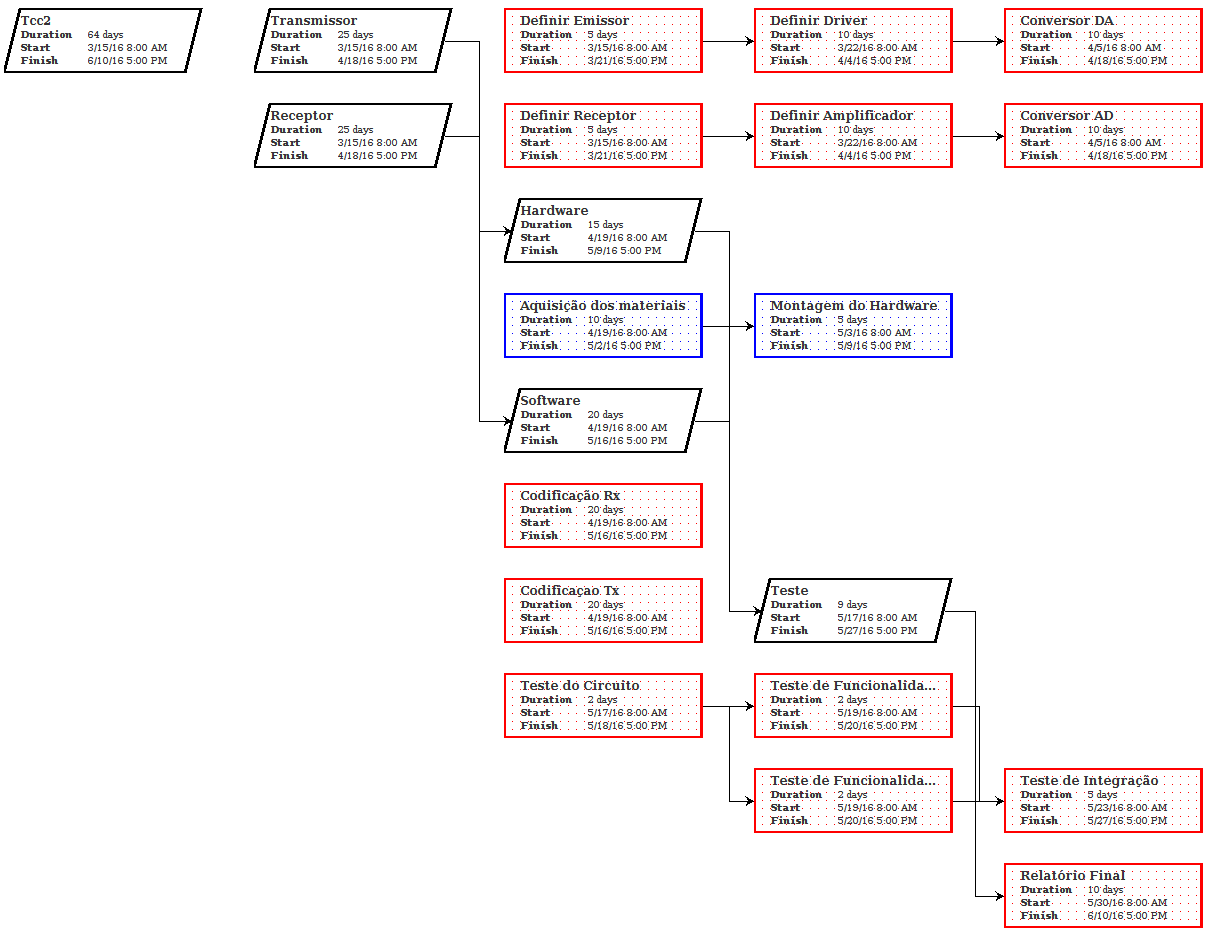
\includegraphics[width = 18cm]{figuras/Network_diagram.png}
	\caption{Diagrama de dependências proposto para o Trabalho de Conclusão de Curso 2.}
	\label{Fig: Network_diagram}
\end{figure}

\begin{figure}
	\centering
		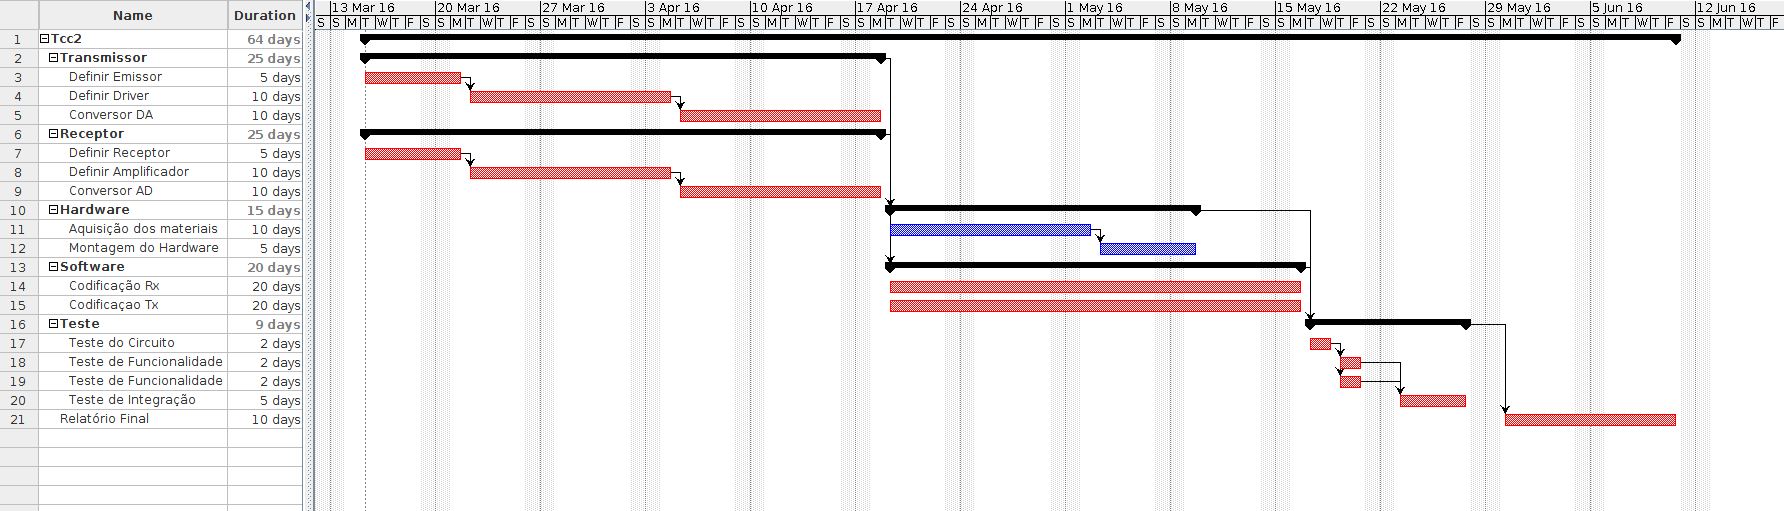
\includegraphics[width = 25cm, angle = 90]{figuras/Grantt_diagram.png}
	\caption{Cronograma proposto para o Trabalho de Conclusão de Curso 2.}
	\label{Fig: Grantt_diagram}
\end{figure}

\end{apendicesenv}
